\documentclass{ieeeaccess}
\usepackage{cite}
\usepackage{amsmath,amssymb,amsfonts}
\usepackage[OT1]{fontenc}
\usepackage{algorithmic}
\usepackage{algorithm2e}
\usepackage{multicol}
\usepackage{graphicx}
\usepackage{textcomp}
\def\BibTeX{{\rm B\kern-.05em{\sc i\kern-.025em b}\kern-.08em
    T\kern-.1667em\lower.7ex\hbox{E}\kern-.125emX}}
\begin{document}
\history{Received December 4, 2018, accepted December 26, 2018, date of publication January 11, 2019, date of current version February 12, 2019.}
\doi{10.1109/ACCESS.2019.2892066}

\title{Phishing Website Detection Based on
Multidimensional Features Driven
by Deep Learning}
\author{\uppercase{PENG YANG,}
\uppercase{GUANGZHEN ZHAO AND PENG ZENG}}
\address[1]{School of Computer Science and Engineering, Southeast University, Nanjing 211189, China}
\address[2]{Key Laboratory of Computer Network and Information Integration Ministry of Education, Ministry of Education, Nanjing 211189, China}

\tfootnote{This work was supported in part by the National Natural Science Foundation of China under Grant 61472080 and Grant 61672155, in part
by the Consulting Project of Chinese Academy of Engineering under Grant 2018-XY-07, and in part by the Collaborative Innovation
Center of Novel Software Technology and Industrialization.}

\markboth
{P. Yang \headeretal: Phishing Website Detection Based on
Multidimensional Features Driven
by Deep Learning}
{P. Yang \headeretal: Phishing Website Detection Based on
Multidimensional Features Driven
by Deep Learning}

\corresp{Corresponding author: Peng Yang (pengyang@seu.edu.cn)}

\begin{abstract}
As a crime of employing technical means to steal sensitive information of users, phishing is currently a critical threat facing the Internet, and losses due to phishing are growing steadily. Feature
engineering is important in phishing website detection solutions, but the accuracy of detection critically depends on prior knowledge of features. Moreover, although features extracted from different dimensions are more comprehensive, a drawback is that extracting these features requires a large amount of time. To address these limitations, we propose a multidimensional feature phishing detection approach based on a fast detection method by using deep learning. In the first step, character sequence features of the given URL are extracted and used for quick classification by deep learning, and this step does not require thirdparty assistance or any prior knowledge about phishing. In the second step, we combine URL statistical features, webpage code features, webpage text features, and the quick classification result of deep learning into multidimensional features. The approach can reduce the detection time for setting a threshold. Testing on a dataset containing millions of phishing URLs and legitimate URLs, the accuracy reaches 98.99\%, and the false positive rate is only 0.59\%. By reasonably adjusting the threshold, the experimental results show that the detection efficiency can be improved.
\end{abstract}

\begin{keywords}
Phishing website detection, convolutional neural network, long short-term memory
network, semantic feature, machine learning.
\end{keywords}

\titlepgskip=-35pt

\maketitle

\section{Introduction}
The Internet has become an indispensable infrastructure
that brings great convenience to human society. However,
the Internet is also characterized by some inevitable security
problems, such as phishing, malicious software, and privacy
disclosure, which have already brought serious threats to
the economy of users. The APWG (Anti-Phishing Working
Group) defines phishing as a criminal mechanism employing
both social engineering and technical subterfuge to steal
personal identity data and financial account credentials of
consumers [1]. Phishing is a very popular method used in
network attacks and leads to privacy leaks, identity theft and
property damage. According to statistics from the Kaspersky
Lab, in 2017, 29.4\% of user computers were subjected to
at least one Malware-class web attack over the year and
199 455 606 unique URLs were recognized as malicious
by web antivirus components [2]. In addition, the share of financial phishing increased from 47.5\% to almost 54\% of
all phishing detections in 2017 [2]. Phishing has become one
of the biggest security threats in the Internet.\par
The spread of phishing is no longer limited to traditional
modalities such as e-mail, SMS, and pop-ups. Though
the prosperity of the mobile Internet and social networks
have brought convenience to users, they have also been
employed to spread phishing, such as QR code phishing,
spear phishing and spoof mobile applications [3]-[5],
etc. In addition, many cunning phishing attacks are hosted
on websites that have HTTPS and SSL certificates because
many users think that HTPPS websites are likely legitimate
[1]. Phishing presents a diversified development trend,
which poses new detection challenges. While phishers
are pernicious and hide, security experts and researchers
have dedicated many efforts in terms of phishing website
detection.\par
Blacklists and whitelists are widely used in phishing
website detection. The current common browsers integrate
blacklists and whitelists to protect users from phishing
attacks. Google provides a blacklist of malicious websites
that is continuously updated. Users can check the security of
URL links through Google Safe Browsing APIs [6]. Phishing
website detection based on blacklists and whitelists is easy
to implement with high running speed and a low false positive
rate. However, according to statistics [7], 47\%-83\% of
phishing websites are added to blacklists after 12 hours, and
63\% of phishing websites have a lifespan of only 2 hours;
thus, the updating of the blacklist is far behind the generation
of phishing websites. In addition to blacklist and
whitelist, machine learning methods are widely used in phishing
website detection [8], [9]. The reason is that malicious
URLs or phishing webpages have some characteristics that
can be distinguished from legitimate websites, and machine
learning can be effective in this regard for processing.
Current mainstream machine learning methods of phishing
website detection extract statistical features from the URL
and the host [10] or extract relevant features of the webpage,
such as the layout, CSS, text [11], [12], and then classify
these features. However, these methods only analyze the
URL or extract features from a single perspective, which
makes it difficult to extract the complete attributes of phishing
websites. Moreover, some unreasonable features may reduce
the accuracy of detection. The character sequence of the
URL is natural, automatically generated feature that avoids
the subjectivity of artificially selected features. In addition,
it does not require third-party assistance and any prior knowledge
about phishing. However, in the process of character
sequencing, the difficulty is to effectively extract association
and semantic information.\par
To address these problems, we propose a multidimensional
feature phishing detection approach based on a fast detection
method by using deep learning (MFPD). In the first step,
character sequence features of the given URL are extracted
and used for quick classification by deep learning. Specially,
the CNN (convolutional neural network) is used to extract
local correlation features through a convolutional layer. In a
URL, each character may be related to nearby characters.
Generally speaking, a phishing website is likely to mimic
the URL of a legitimate website by changing or adding some
characters. This can cause the sequential dependency of the
phishing URL to be different from the phishing URL. The
LSTM network can effectively learn the sequential dependency
from character sequences. Therefore, the LSTM (long
short-term memory) network is employed to capture context
semantic and dependency features of URL character
sequences, and at finally softmax is used to classify the
extracted features. We call the first step CNN-LSTM. From
a comprehensive perspective, in the second step, we combine
URL statistical features, webpage code features, webpage
text features and the classification result of deep learning
into multidimensional features, which are then classified by
XGBoost. Although the multidimensional feature detection method has higher accuracy, it requires extracting features
from different aspects, resulting in longer detection time.
In contrast, the method for the URL character sequences
only needs to process the URL, and the detection time is
short. To balance the contradiction between detection time
and accuracy, we improve the output judgment condition of
the softmax classifier in the deep learning process by setting
a threshold to reduce the detection time. If the result of deep
learning is not less than the specified threshold, the detection
result is directly output; otherwise, go to the second step of
detection.\par In particular, our key contributions in this work are listed
as follows:
\begin{itemize}
  \item With the phishing website detection as a two-category
processing model, we formally define the problem of
phishing detection and give a specific formal description
of the MFPD approach.
  \item We build a real dataset by crawling a total of 1 021
758 phishing URLs as positive samples from phishtank.
com, and a total of 989 021 legitimate URLs as
negative samples from dmoztools.net.
  \item The process of phishing website detection using MFPD
is explained, and an extensive experiment on the dataset
we built is conducted. The results show that our proposed
approach exhibits good performance in terms of
accuracy, false positive rate, and speed.
  \item A dynamic category decision algorithm (DCDA) is proposed.
By revising the output judgment conditions of
the softmax classifier in the deep learning process and
setting a threshold, the detection time can be reduced.
\end{itemize}\par
The paper is organized as follows. In Section II,
we present related work on phishing website detection.
Then, in Section III, we introduce the framework of MFPD.
In Section IV, we describe the detailed process of the MFPD,
which includes the CNN-LSTM and multidimensional features.
The performance of the proposed approach is evaluated
in Section V. Finally, in Section VI, we conclude the paper
and discuss future work.
\section{Related Work}
In this section, we describe the phishing website detection
method based on machine learning, including traditional
methods and deep learning methods.\par The phishing website detection based on machine learning
is a hotspot of current phishing website detection
research. The results of machine learning methods usually
depend on the quality of the extracted features. The focus of
current research is on how to extract and select more effective
features before processing them.\par Resources on the Internet are addressed by URLs, which
consist of the Hostname and FreeURL. The typical URL
structure is shown in Fig. 1. \par Considering a phishing URL that imitates PayPal ``http://
cancellation-paypal.us-com.15ffe4fd8f.com/signin/'' as an
example. The structure is as follows:
\begin{itemize}
    \item Protocol: http
    \begin{figure}
        \centering
        
\includegraphics[width=\linewidth]{Figure1.png}
        \caption{The typical structure of a URL.}
        \label{fig:1}
    \end{figure}
    \item Subdomain: cancellation-paypal.us-com
    \item Domain : 15ffe4fd8f.com
    \item Hostname: cancellation-paypal.us-com.15ffe4fd8f.com
    \item FreeURL: /signin/
\end{itemize}\par Phishers generally distort the hostname part and the path
part from the URL of the target webpage to generate the
phishing URL, and therefore, features can be extracted based
on URL statistical rules [13], [14] or simply based on the
URL strings [15]. Researchers have proposed many unique
features of different types of phishing websites from different
perspectives.\par Zouina and Outtaj [9] proposed a lightweight phishing
website detection method that used only six URL features,
namely, the URL size, the number of hyphens, the number
of dots, the number of numeric characters plus a discrete
variable that corresponds to the presence of an IP address
in the URL, and finally, the similarity index. The features
extracted are completely based on URLs, and because of their
low features, the detection speed is fast. However, the amount
of experimental data was relatively small.\par Le et al. [15] proposed a method of extracting lexical features
from URL strings and using AROW(Adaptive Regularization
of Weights) to detect phishing websites. This method
overcomes the noise of the training data while ensuring detection
accuracy.\par Verma and Dyer [16] innovatively proposed KS
(Kolmogor-ov-Smironov) distance, KL (Kullback-Leibler
Divergence) distance, Euclidean distance, character frequency
and editing with the target URL based on the difference
in characters between the phishing URL and standard
English, combining these features with URL features.\par Phishing detection mechanisms based on the URL feature
only need to process the URL, and thus, the detection speed
is fast. However, the URL information alone does not fully
represent the characteristics of phishing websites. Current
research generally extracts HTML and text features of webpages
[17], third-party site features [18], etc., and combine
these features with URL features to develop multidimensional
features.\par Xiang et al. [19] proposed the CANTINAC phishing website
detection framework based on CANTINA. The method
first filtered out highly similar phishing websites and webpages
without login forms and then extracted 15 highly differentiated
features from URL vocabulary, HTML DOM,
WHOIS information and search engine information, finally
implementing phishing website prediction using a machine
learning algorithm.\par Marchal et al. [20] proposed a scalable and languageindependent
phishing website detection method. In terms
of URL and HTML, 212 features were selected; Gradient
Boosting was used to detect phishing websites and yielded
a high accuracy. Phishing detection based on the combined
features more fully represents the website, and therefore,
the detection effect is better. However, it is necessary to download
a webpage or obtain data from a third-party website, and
there some issues remain, namely, that the feature extraction
is complicated, and real-time detection cannot be satisfied.\par After extracting features, phishing website detection is
generally considered to be a clustering or classification
problem. Cluster-based phishing website detection does not
require labeled phishing samples or legitimate samples. The
clustering algorithm divides features into several clusters
such that the similarity of samples within the same cluster
is higher, and the similarity of samples in different clusters
is lower. Finally, the different clusters are used to distinguish
legitimate and phishing websites [21]-[23]. The cluster-based
phishing website detection method reduces the cost of manually
labeling the dataset, but the detection result is highly
dependent on the quality of the features, and the accuracy is
not high [24].\par The current phishing detection method based on machine
learning mainly uses a supervised classification algorithm to
detect the legitimacy of websites. The classification model
introduces the marked website dataset, trains the existing
classification model with a training dataset, and predicts
the legitimacy of websites through the trained classifier.
Current popular classification models are LR (logistic regression),
SVM (support vector machine), NB (naïve Bayes), RF
(random forest), neural network, etc., and the corresponding
revised algorithms [25]-[28].\par Ma et al. [25] extracted integer features, binary features
and host features based on the phishing URL and then compared
the detection performance of multiple classifiers. The
results showed that LR had the fastest running speed while
ensuring accuracy.\par Mohammad et al. [26] proposed an intelligent model for
predicting phishing attacks based on artificial neural networks,
particularly, self-structuring neural networks. This
neural network model first established a minimized threelayer
neural network in which the hidden layer has only
one neuron and then gradually increased the hidden layer
neurons through feedback on model training. This model
makes full use of the advantages of neural networks, has good
acceptance for noise data and good generalization ability.
However, it cannot automatically extract deep features, and
the classification results are highly dependent on the features
that have been extracted.\par Deep learning is a research direction of neural networks
that can discover hidden information within complex data
through level-by-level learning. CNN is a deep feedforward
artificial neural network. Compared with traditional backpropagation
neural networks [29], CNNs adopt a weightsharing
network structure similar to that of a biological neural network, and its neurons are sparsely connected, which
reduces the complexity of the network model and improves
training performance.\par Traditional neural network models are not suitable for
processing time series problems, while RNN (Recent Neural
Network) is good at dealing with time series problems of
data with learning the previous information [30]. The current
output is not only related to the current input but also
related to the previous output. The LSTM (long short-term
memory) network is an improved version of the traditional
RNN model, which can solve the long-distance dependence
problem caused by ``gradient dispersion'' in the RNN.\par At present, there are some studies on phishing website
detection based on deep learning. Selvaganapathy et al. [31]
proposed a phishing URL detection algorithm using stacked
restricted Boltzmann machine for feature selection and deep
neural networks as classifiers. Then, multiple detections were
constructed using IBK-kNN, Binary Relevance, and Label
Powerset with SVM. This model improves the accuracy of
detection by combining the recognition results of multiple
classifiers. Bahnsen et al. [32] extracted the syntax and statistical
characteristics of the URL, and then classified the
character sequence of the URL using LSTM. By comparing
with RF, experiments showed that LSTM was better than RF.\par Based on the above analysis, we regard the URL strings
as URL character sequences, which are natural features that
do not require prior knowledge about phishing. In the processing
of URL character sequences, we refer the idea of
the literature [33] to treat the URL as a sequence of text
string and quantize the URL at the character level. Therefore,
we take advantages of CNN to extract the local features of the
sequence, and then use take advantages of LSTM to extract
the context semantic features of the sequence, and finally the
extracted features are classified by softmax.
\section{PROPOSED ARCHITECTURE}
In this section, we first define the formal statement of phishing
website detection, then describe the overall framework of
the approach MFPD and its formal definition.

\subsection{PROBLEM STATEMENT}
Suppose we are given a set U consists of all URLs. Then 
$U=\left\{u\left|u=x_{i}, x_{i} \in\right| u r l, i \in N^{+}\right\},|U|=n$ Let $C_{p}$ as a set indicating phishing, 
set indicating phishing, $C_{p}=\{c | c=p, p \in \text {phishing}\}$, $C_{l}$ as
a set indicating legitimate, $C_{l}=\{c | c=l, l \in \text {legitimate}\}$, and $C=C_{p} \cup C_{l}$, $u_{i}$ is a suspicious URL. Formally, phishing
website detection problem can be defined as follows:\vspace{6pt} \par \textit{Definition 1 (Phishing Detection of $u_{i}$):} Let P(C) as the
power set of C, the time cost of detecting $u_{i}$ is $tc_{i}$.Defining
function t : $U \rightarrow P(C)$, t as a mapping relationship needs
to be found to implement the detection of $u_{i}$ Let $C_{i}^{\prime}$ as the calculated result by t, and $C^{\prime}=\cup_{i \in n} C_{i}^{\prime}$, $C_{i}$ as the category to the URL $u_{i}$, $C_{i} \in C$ obviously $C_{i}=\left\{\begin{array}{ll}{0} & {\text { legitimate }} \\ {1} & {\text { phishing }}\end{array}\right.$. We can describe phishing website detection as: \vspace{6pt}
\par
\begin{equation}
\forall u_{i} \in D, \quad C_{i}^{\prime}=t\left(u_{i}\right)
\end{equation}
The objective function is:
\begin{equation}
O(u)=\max \left(n-\sum_{i=1}^{n}\left(t\left(u_{i}\right) \oplus C_{i}\right) / \sum_{i=1}^{n} t c_{i}\right)
\end{equation}\par The essence of solving the phishing website detection
problem is to find a suitable function t such that the objective
function obtains the maximum value.
\subsection{THE FRAMEWORK OF MFPD}
In this paper, we built the framework of the proposed
approach, referred to as MFPD. MFPD can be described by
the following four definitions.\vspace{6pt} \par \textit{Definition 2 (Character embedding of $u_{i}$):} Let the fixed length of the URL $u_{i}$ be L, then $m=97 \times L$ according to Table 1. For $u_{i}$, the length of the URL character sequence is
unified based on the formula (5)$e_{i}$ = URLF($u_{i}$) and encoded
based on Table 1 $g_{i}$ = ASC($e_{i}$). Then, regarding $g_{i}$ as a vector
and $\overrightarrow{g_{i}}=\left(g_{i}^{1}, g_{i}^{2}, \ldots, g_{i}^{j}\right)^{T}, g_{i}^{j}$. Finally, the embedding
network is used to reduce the sparsity of G. Letting the
network weight be $V, V \in \mathbb{R}^{p \times m}$, the result of character
embedding is: \begin{equation}
\begin{aligned} S &=V G=\left[\begin{array}{ccc}{v_{11}} & {\dots} & {v_{1 m}} \\ {\vdots} & {\ddots} & {\vdots} \\ {v_{p 1}} & {\cdots} & {v_{p m}}\end{array}\right] \times\left[\begin{array}{ccc}{g_{11}} & {\dots} & {g_{1 n}} \\ {\vdots} & {\ddots} & {\vdots} \\ {g_{m 1}} & {\cdots} & {g_{m n}}\end{array}\right] \\ &=(\overrightarrow{s_{1}}, \overrightarrow{s_{2}}, \dots, \overrightarrow{s_{n}}) \end{aligned}
\end{equation} and $S \in \mathbb{R}^{p \times n}$. The process of character embedding is $T: U \rightarrow S$.

\begin{table}[htp]
\caption{Character Map}
\label{table:1}
\begin{tabular}{llll}
\hline
Characters                                                                            &  &  & Encode \\ \hline
abcdefghijklmnopqrstwxyz                                                              &  &  & 1-26   \\
ABCDEFGHIJKLMNOPQRSTWXYZ                                                              &  &  & 27-52  \\
0123456789                                                                            &  &  & 53-62  \\
-,.!?;"'\textasciicircum{}@\#\$\%\&*$\sim$`+=-\_\textless{}\textgreater{}()\{\}{[}{]} &  &  & 63-95  \\
default                                                                               &  &  & 0      \\
unknow                                                                                &  &  & 96     \\ \hline
\end{tabular}
\end{table}\par \vspace{4pt}
\textit{Definition 3 (CNN-LSTM):} Let W be the weight of
the CNN-LSTM network. $C^{\prime \prime}$ is the result of CNN-LSTM
processing.\par For the set $U, U=U_{\text {train}} \cup U_{\text {test}}$ and $U_{\text {train}} \cap U_{\text {test}}=\emptyset$ The training and testing processes for this network are:\par \vspace{4pt} $\operatorname{Train}\left(\cup_{i \in t} u_{i}, \cup_{i \in t} C_{i}\right) \rightarrow W$,   $u_{i} \in U_{\text {train }}, \quad\left|U_{\text {train}}\right|=t$,\par \vspace{4pt} $\operatorname{Test}\left(\cup_{j \in h} u_{j}, W\right) \rightarrow C^{\prime \prime}$,   $u_{j} \in U_{\text {test}}, \quad\left|U_{\text {test}}\right|=h$.\par Therefore, the CNN-LSTM can be described as follows:\par \vspace{4pt} $\begin{aligned} S_{\text {train}} &=T\left(U_{\text {train}}\right), \quad S_{\text {test}}=T\left(U_{\text {test}}\right) \\ C^{\prime \prime} &=\text {Test }\left(S_{\text {test}}, T r a i n\left(S_{\text {train}}, \nu_{j \in h} C_{j}\right)\right), \quad\left|S_{\text {train}}\right|=h \end{aligned}$
\begin{figure*}[ht]
        \centering
        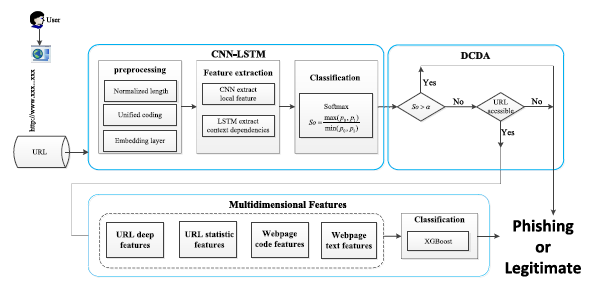
\includegraphics[width=\linewidth]{figure2.png}
        \caption{The framework of MFPD.}
        \label{fig:2}
    \end{figure*}
\par \textit{Definition 4 (Multidimensional Features):} Let the URL
statistical features be defined as set Fu, the webpage code
features be set Fc, and the webpage text features be set Ft. For $C^{\prime \prime}$ obtained from CNN-LSTM, the multidimensional
features are: \vspace{2pt} \par
$F=C^{\prime \prime} \cup F u \cup F C \cup F t, \quad F^{\prime}=X G B o o s t(F)$
\par \textit{Definition 5 (DCDA):} We revised the softmax in the
CNN-LSTM. Let $p_{0}$ be the probability of a legitimate website
output by the softmax, while $p_{1}$ is the probability of a
phishing website output, and let $\alpha$ be the threshold.\par
\begin{equation}
S o=\frac{\max \left(p_{0}, p_{1}\right)}{\min \left(p_{0}, p_{1}\right)}, \quad p_{1}=1-p_{0}
\end{equation}
\par if $s_{0} > {\alpha}$ or $d_{i} {\in} unaccessible, C^{\prime} = arg max(p_{0}, p_{1})$; otherwise, go to the Multidimensional Features.\par
The framework of our proposed approach is divided into
three modules, as shown in Fig. 2. The first is the CNNLSTM
module, which contains data preprocessing, feature
extraction and classification. The data consists of a large
number of legitimate and phishing URLs collected from the
Internet. The URL character sequences are preprocessed,
which includes length normalization, uniform encoding, and
using an embedding layer to reduce the sparsity of the data.
In feature extraction, theCNNis used to extract local features,
and LSTM is used to extract context dependency. We use
softmax to classify the clean-up features. The second module
defines the Multidimensional Features, which are based on
URL statistical features, webpage code features, webpage
text features. The result of the CNN-LSTM is then used by
XGBoost for classification. The second module has greater
accuracy than the CNN-LSTM module but also has more time cost. Therefore, to achieve real-time detection, at the last
module DCDA, we improve the classification output of the
softmax classifier. The threshold is used to determine whether
to focus on accuracy or real-time detection. Moreover, when
the URL is unreachable, the output of softmax is directly used
as the result of the detection.
\section{OVERVIEW OF ALGORITHM}
In this section, we introduce in detail the process of data
preprocessing and the construction and training of the
CNN-LSTM algorithm, the phishing detection method based
on multidimensional features, and the optimization strategy
DCDA for balancing accuracy and speed.\vspace{6pt}
\subsection{THE CNN-LSTM ALGORITHM}
The CNN-LSTM algorithm contains three parts as shown
in Fig. 3: URL embedded representation, feature extraction,
classification. \par At the embedded representation stage of the URL, the URL
character sequence is normalized to a fixed-size sequence by
intercepting or zero-filling, and then, the normalized string is
converted into a one-hot code sequence according to Table 1.
Then, the sparse one-hot matrix is converted into a dense
character embedding matrix through the embedding layer.
In the feature extraction stage, the local deep correlation
feature is extracted from the embedding matrix through the
convolutional layer and maximum pooling of the CNN. Then,
the result of the pooling is input to the LSTM neural network
to capture the context of the URL sequence. In the classification
stage, the output of the last moment of the LSTM neural
network is input to the softmax unit. To prevent overfitting,
\begin{figure}
    \centering
    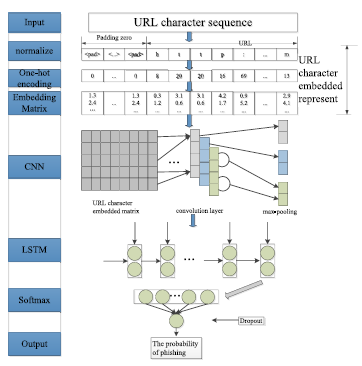
\includegraphics[width=\linewidth]{figure3.png}
    \caption{The CNN-LSTM algorithm.}
    \label{fig:3}
\end{figure}
a dropout strategy is used, and softmax outputs the probability
that the URL belongs to a phishing website.\par
The URL character embedded representation achieves
transformation of the URL string into a data matrix that the
model can recognize. To do this, we assume that the length
of each URL character is fixed to L. If the URL length
exceeds L, the extra characters are intercepted at the end of
the URL. If the URL length is less than L, zeros are added
to the URL header until the length reaches L. We define the
function as $URLF : U {\in} E$, where D indicates the raw URL,
and E indicates the normalized URL. The specific description
is \par
\begin{equation}
U R L F(u)=\left\{\begin{array}{ll}{P A D+u_{i},} & {\operatorname{len}\left(u_{i}\right)<L} \\ {u_{i},} & {\operatorname{len}\left(u_{i}\right)=L} \\ {u_{i}[0: L-1],} & {\operatorname{len}\left(u_{i}\right)>L}\end{array}\right.
\end{equation}
where $len(u_{i})$ indicates the length of the URL $u_{i}$ and PAD is
a zero-padded string with length $len (PAD) = L- len(u_{i})$, and $u_{i}[0:L-1]$ is the first L characters of the URL $u_{i}$. \par All letters, numbers, and special characters that may appearin the URL are determined, and the character mappingrules are built. According to the ASCII code table and the
actual situation of the URL characters, a 97-number-character
mapping table is constructed, including 52 uppercase and
lowercase letters, 10 numbers, 33 feature characters, one
zero-padded character and an unknown character number.
We define the mapping as $ASC : E {\rightarrow} G$, where E indicates
the original character, and G indicates the number encoded.
The character mapping table is shown in Table 1.\par According to Table 1, the header zero-padded character corresponding to the number is 0, and the character ``0'' corresponds to the number 53; finally, each character is converted
into a one-hot fragment $g^{\prime}$ of length 97, in which the position corresponding to the character is 1, and the rest of the positions are 0. For example, the character ``a'' is represented as $g^{\prime}=(0,1,0, \ldots, 0)$ The integral URL $u_{i}$ s converted to the vector $\overrightarrow{g_{i}}$, defined as \par \begin{equation}
\overrightarrow{g_{i}}=\left(g_{1}^{\prime}, g_{2}^{\prime}, \ldots, g_{L}^{\prime}\right)^{T}, \quad|\overrightarrow{g_{i}}|=m=97 \times L
\end{equation} \par Since the one-hot encoded vector $\overrightarrow{g_{i}}$ contains many zeros, it will cause sparse coding and high dimensionality, and
there is no spatial and semantic correlation between different
characters in $\overrightarrow{g_{i}}$. Fortunately, this problem can be solved by
converting it into a low-dimensional dense character embedding
space. In this paper, each one-hot vector $\overrightarrow{g_{i}}$ is projected
into the p-dimensional continuous vector space $\mathbb{R}^{P}[34]$ 
Corresponding to the embedded layer in the neural network, it can
be understood as a fully connected neural network with input
neurons of m and output neurons of p. The embedded layer is
shown in Fig. 4.
\begin{figure}
    \centering
    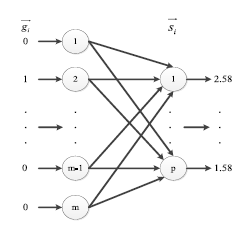
\includegraphics[width=\linewidth]{figure4.png}
    \caption{The embedded layer}
    \label{fig:4}
\end{figure}
\par Let its parameter matrix be $V, V \in \mathbb{R}^{p \times m}$, then for the
one-hot vector $\overrightarrow{g_{i}}$, its final embedding vector $\overrightarrow{s_{i}}$ is \par
\begin{equation}
\begin{aligned} \overrightarrow{s_{i}} &=V \overrightarrow{g_{i}}=\left[\begin{array}{ccc}{v_{11}} & {\cdots} & {v_{1 m}} \\ {\vdots} & {\ddots} & {\vdots} \\ {v_{p 1}} & {\cdots} & {v_{p m}}\end{array}\right] \times\left[\begin{array}{c}{g_{i 1}} \\ {\vdots} \\ {g_{i m}}\end{array}\right] \\ &=\left(s_{i 1}, s_{i 2}, \ldots, s_{i p}\right)^{T} \end{aligned}
\end{equation}\par
Let all URLs form matrix $G=G_{m \times n}=(\overrightarrow{g_{1}}, \overrightarrow{g_{2}}, \ldots, \overrightarrow{g_{n}})$, so all the URLs string are converted to a dense matrix S = VG = $(\overrightarrow{s_{1}}, \overrightarrow{s_{2}}, \ldots, \overrightarrow{s_{n}})$ and $S \in \mathbb{R}^{p \times n}$, which is the character embedding matrix of the URL.
\par After preprocessing, we get dense representation of the raw
URL character sequence S. The convolution layer in CNN
performs convolution operation on S to extract local deep
associated features. Specifically, the convolution layer sets a
plurality of convolution kernels Q, each of which convolves
a character embedding vector having a window size of k to
produce new features. For the f -th convolution kernel, its
character embedding matrix $E_{i}$ at the i-th sliding window is $E_{i}=(\overrightarrow{s_{i}}, \overrightarrow{s_{i+1}}, \ldots, \overrightarrow{s_{i+k-1}})$. Then, the new feature computed
by the convolution kernel f at the i-th sliding window is $h_{i}^{f}=\sigma\left(W_{f} \cdot E_{i}+b_{f}\right)$, where $\sigma(x)$ is a ReLU activation function, which represents the nonlinear activation function of the convolutional layer, $W_{f} \in \mathbb{R}^{p \times k}$ is the weight matrix
of the convolution kernel, $b_{f}$ is the bias.
\par We set the sliding step size is 1, and the feature vector generated
by the convolution kernel f computing the sliding window $E_{0}$ to $E_{L-k+1}$ is $\vec{h}^{f}=\left(h_{1}^{f}, h_{2}^{f}, \ldots, h_{L-k+1}^{f}\right)^{T}$. Stacking the feature generated by the Q convolution kernels to obtain a new sequence matrix $H_{s}=(\overrightarrow{h_{1}}, \overrightarrow{h_{2}}, \ldots, \overrightarrow{h_{i}}, \ldots, \overrightarrow{h_{s}})^{T}$, $\overrightarrow{h_{i}} \in \mathbb{R}^{N \times 1}$ The pooling layer performs Max-Pooling operation on the new sequence matrix $H_{s}$ to obtain the
maximum value of the pooling window with size of k,
thereby maximizing the character feature representation.
We set the pooling step size to the same as the pooling
window. After conducting the Max-Pooling operation
on the vector $\overrightarrow{h^{f}}$ and vector $\overrightarrow{p^{f}}$ is obtained. $\overrightarrow{p^{f}}=\left(p_{1}^{f}\right.$, $\left.p_{2}^{f}, \ldots, p_{j}^{f}, \ldots, p_{N}^{f}\right)^{T}$, where $p_{j}^{f}$ is value of the j-th Max-Pooling, $p_{j}^{f}=\operatorname{Max}\left(h_{(j-1) p}^{f}, h_{(j-1) p+1}^{f}, \ldots, h_{j p-1}^{f}\right)$, N = $\lceil(L-k+1) / p\rceil$ Finally, the pooled sequence matrix $H_{p}$ \par $H_{p}=(\overrightarrow{p^{1}}, \overrightarrow{p^{2}}, \ldots, \overrightarrow{p^{j}}, \ldots, \overrightarrow{p^{s}})^{T}, \quad \overrightarrow{p^{j}} \in \mathbb{R}^{N \times 1}$ \vspace{6pt} \\ can be obtained by stacking S pooling vectors. \par After that, the pooled sequence matrix $H_{p}$ is input into the LSTM neural network, $p^{i}$ as the input of the LSTM network at the i-th moment. and LSTM outputs the hidden
state sequence $H =(\overrightarrow{h_{1}}, \overrightarrow{h_{2}}, \ldots, \overrightarrow{h_{N}})$ Then, put the last
hidden state $\overrightarrow{h_{N}}$ of the sequence into the softmax classifier,
which uses the regression unit with the sigmoid activation function to classify. The prediction probability is as shown follows. \par 
\begin{equation}
p(y=k | X)=\frac{\exp \left(w_{k} x+b_{k}\right)}{\sum_{i=0}^{k-1} \exp \left(w_{i} x+b_{i}\right)}
\end{equation}\par
When k = 0, it indicates the probability of belonging
to a legitimate website, and when k = 1, it indicates the
probability of belonging to a phishing website.
\par To suppress overfitting, the dropout strategy is applied in
the fully connected layer between the $h_{N}$ and softmax classification. Dropout is an efficient strategy to prevent overfitting in deep neural networks [35], [36], which discards each neural network unit from the network with a certain probability during training, as shown in Fig. 5.\begin{figure}
    \centering
    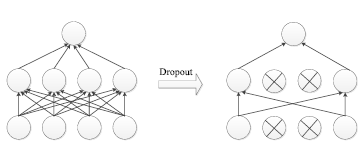
\includegraphics[width=\linewidth]{figure5.png}
    \caption{The dropout strategy.}
    \label{fig:5}
\end{figure} \par The key to training the model is determining the target loss
function. We use the cross-entropy loss function, as shown follows. \vspace{6pt} \par \begin{equation}
L(\widehat{y}, y)=-\frac{1}{N} \sum_{i}^{N}\left[y_{i} \log \widehat{y_{i}}+\left(1-y_{i}\right) \log (1-\widehat{y_{i}})\right]
\end{equation}
\vspace{6pt} \par The optimization method of the loss function is to constantly
adjust the weights in the neural network during the
iterative process of the model. A commonly used optimization
strategy is the SGD (stochastic gradient descent) algorithm,
which calculates each sample gradient and updates
the parameters during the training process. Frequently updating
the parameters by SGD will result in the loss function
generating severe oscillations, the minimum value of the
loss function may not be obtained, and the function could
easily fall into a local minimum. Adam (adaptive moment
estimation) is an improvement of the SGD algorithm. Adam
calculates the independent adaptive learning rate for different
parameters by calculating the first moment estimation and the
second moment estimation of the gradient. Compared with
other algorithms, Adam avoids the problems of the learning
rate disappearing, slow convergence, and great fluctuations in
the loss function [37].\par The CNN-LSTM training and testing process is shown as
follows.\vspace{6pt}
\subsection{THE MULTIDIMENSIONAL FEATURE ALGORITHM}
The URL character embedding matrix cannot fully represents
the phishing website information. In this section, we combines
URL statistical feature, webpage code feature, webpage
text feature and the quick classification result of CNN-LSTM
into multidimensional features and describes the overall flow
in detail.
\par To confuse users, phishers generally imitate the URL of
the target website to produce a phishing URL. For example,
in order to imitate the URL of the PayPal website, the phishing
URL appears to have a PayPal in its subdomain name, and
its domain name is disorderly. According to the above URL
structure in Fig. 1, 20 kinds of URL statistical features are
extracted. In addition, the phishing webpage has manyHTML
source code and JavaScript source code exceptions, such as
more external links and empty links, empty form actions,
and more pop-up windows. Reasonable use of these features
can effectively identify phishing, so we extract 24 kinds of
webpage code features, as shown in Table 2.
\par In Table 2, the Information entropy refers to the uncertainty
of URL characters. The Euclidean distance is used to calculate
the similarity between the frequencies of URL character
and standard English character, and the Kullback-Leibler
divergence represents the relative entropy of both above.
The Edit distance outlier shows the similarity between the
phishing website and the legitimate website that is imitated
by a phisher. Calculations or regular expression matching is
employed to extract webpage code features from HTML and
JavaScript code, respectively, which represents the number of
tags and functions in the webpage source code.
\begin{table}[htp]
\begin{tabular}{l}
\hline
\textbf{Algorithm 1} The CNN-LSTM Algorithm                                                                                                                                                                                                                         \\ \hline
\textbf{Input:} The training set $U_{train}$, the testing set $U_{test}$, $u_{i}\in$ \\ $S_{train}, u_{i}^{\prime} = S_{test}$.                                                                                           \\
\textbf{Output:} The probability of phishing $P(u_{i}^{\prime}).                                                                                                                                                              \\
1: K = num of sliding-window, k = size of sliding step,\\
    p = size of pooling-window, $\beta$ = threshold of the loss\\
    function L(x,y). $Weight_{embedding} = V$, $V \in \mathbb{R}^{p \times m}$,
    $G \in \mathbb{R}^{m \times n}$.                                                                                                                                                                                           \\
    
2: $U=U_{\text {train}} \cup U_{\text {test}}, l=|U|, G=\emptyset, N=\lceil K / p\rceil$
                            \\
3: \textbf{for} i in l \textbf{do}                                                                                                                                                                                                                \\
4: $u_{i} \in U, e_{i} = URLF(u_{i})$                                                                                                                                                                                                                                               \\
5: $g_{i} = Asc(e_{i})$                                                                                                                                                                                                                                                              \\
6: $G = G \cup g_{i}$                                                                                                                                                                                                                                                                \\
7: \textbf{end for}                                                                                                                                                                                                                                                \\
8: $S = VG = (\overrightarrow{s_{1}}, \overrightarrow{s_{2}}, \ldots, \overrightarrow{s_{n}})$                                                                                                                                                                                       \\
9: \textbf{for f} in Q do                                                                                                                                                                                                                                         \\
10: \hspace{3pt} \textbf{for i} in C do                                                                                                                                                                                                           \\
11: \hspace{6pt} $h_{i}^{f}=\sigma\left(W_{f} \cdot(\overrightarrow{s_{i}}, \overrightarrow{s_{i+1}}, \ldots, \overrightarrow{s_{i+k-1}})+b_{f}\right)$                                                                                                           \\
12: \hspace{3pt} \textbf{end for}                                                                                                                                                                                                                 \\
13: \textbf{end for}                                                                                                                                                                                                                                               \\
14: \textbf{for f} in Q do                                                                                                                                                                                                                                          \\
15: \hspace{3pt} \textbf{for k} in N do                                                                                                                                                                                                            \\
16: \hspace{6pt} $p_{j}^{f}=\operatorname{Max}\left(h_{(j-1) p}^{f}, h_{(j-1) p+1}^{f}, \ldots, h_{j p-1}^{f}\right)$                                                                                                                                               \\
17: \hspace{3pt} \textbf{end for}                                                                                                                                                                                                                 \\
18: \textbf{end for}                                                                                                                                                                                                                                               \\

19: $H_{p}=\left(\vec{p}^{1}, \vec{p}^{2}, \ldots, \overrightarrow{p^{j}}, \ldots, \overrightarrow{p^{s}}\right)^{T}, \overrightarrow{p^{j}} \in \mathbb{R}^{N \times 1}$                                                                                                         \\

20: $H=\left(h_{1}, h_{2}, \ldots, h_{N}\right)=\operatorname{lstm}\left(H_{p}\right)$                                                                                                                                                                                              \\
21: $C^{\prime \prime} = softmax(h_{N})$                                                                                                                                                                                                                                             \\
22: \textbf{while} $L(C^{\prime \prime}, C) > \beta$\beta$                                                                                                                                                                                                                \\
23: $W = Train (u_{i}, C_{i})$                                                                                                                                                                                                                                                       \\

24: \textbf{end while}                                                                                                                                                                                                                                            \\

25: $P(d_{i}^{\prime}) = Test(u_{i}^{\prime})$                                                                                                                                                                                                                                       \\
26: \textbf{return} $P(u^{\prime})$                                                                                                                                                                                                                                 \\ \hline

\end{tabular}
\end{table}

\par Phishers usually imitate the text content of the target website
to deceive the user. Therefore, it is necessary to extract
the text features of the webpage. The key of this step are
extraction of the effective webpage content and the vectored
representation of the text. To obtain valid text information
in the webpage, we remove the extra parts of the webpage
through regular expressions, including JavaScript code, CSS
code and label characters. A vector space model is employed
to vectorize text of the webpage. The text vector generation
process is shown in Fig. 6. It should be noted that the vectorized
text features usually have large redundant attributes,
which will greatly reduce the efficiency of XGBoost classification. Therefore, we use Logistic regression to train the text vector and generate the probability that the text belongs from the phishing website, then the probability is employed
to represent the webpage text features.
\par After extracting features from different aspects, these features
should be fused. In this paper, the output of CNN-LSTM
algorithm is used as the deep URL features, and it is combined
with the URL statistical features, webpage code features and
\begin{table}[htp]
\caption{URL and webpage code features.}
\label{table:2}
\begin{tabular}{ll}
\hline
URL statistical features                    & Webpage code features \\ \hline
IP address                                  & html\_len              \\
HTTPS protocol                              & div                   \\
URL length                                  & embed                 \\
Length ratio                                & iframe                \\
Containing the "@"                          & applet                \\
Contaiting the "-"                          & frame                 \\
Number of special characters                & input                 \\
Number of dots                              & form                  \\
Number of URL path                          & get                   \\
Length of the longest word in the host name & post                  \\
Longest number length in the host name      & open                  \\
Number of sensitive words:                  & script                \\
Number of top-level domains in paths        & script\_len            \\
Information entropy                         & javascript\_count      \\
Euclidean distance                          & interval              \\
Kullback-Leibler divergence                 & timeout               \\
Edit distance outlier                       & onload                \\
Registration time                           & onerror               \\
Number of domain name servers               & pop                   \\
Alexa ranking                               & exec                  \\
--- ---                                     & dispatchevent         \\
--- ---                                     & eval                  \\
--- ---                                     & attachment            \\
--- ---                                     & externalLinks         \\ \hline
\end{tabular}
\end{table}
\begin{figure}
    \centering
    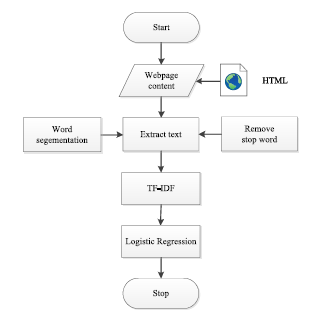
\includegraphics[width=\linewidth]{figure6.png}
    \caption{Text features generation process.}
    \label{fig:6}
\end{figure}
\begin{figure}
    \centering
    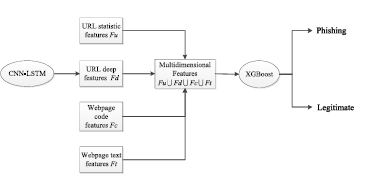
\includegraphics[width=\linewidth]{figure7.png}
    \caption{Multidimensional feature algorithm.}
    \label{fig:7}
\end{figure}
webpage text features to make up multidimensional features,
which are classified by a machine learning approach. The
detailed description is shown in Fig. 7.
\par The classifier used in the multidimensional feature
algorithm is the XGBoost (eXtreme Gradient Boosting)
ensemble learning algorithm, which has high classification
accuracy. XGBoost performs a second-order Taylor expansion
on the loss function, with making full use of the firstorder
and second-order derivatives, and finds the optimal
solution for the regular term outside the loss function, which
improves the classification accuracy. In addition, XGBoost
can automatically utilize a multithreaded CPU for the calculation,
greatly reducing the running time. The detailed process
of the algorithm is as follows:
\begin{table}[htp]
\begin{tabular}{l}
\hline
\textbf{Algorithm 2} The Multidimensional Feature Algorithm                                                                                                                                                                                                                         \\ \hline
\textbf{Input:} The URL set $U, U=\left\{u_{1}, u_{2}, \ldots, u_{n}\right\}$                                                                                           \\
\textbf{Output:} The probability of phishing P(U)                                                                                                                                                              \\
1: $N=|U|, H=\emptyset$                                                                                                                                                                                           \\
    
2: \textbf{for} i in N do \\

   \hspace{12pt} $F d=\emptyset, F u=\emptyset, F c=\emptyset, F t=\emptyset, F=\emptyset$
                            \\
3: \hspace{4pt} $FD = CNN-LISTM(u_{i}$                                                                                                                                                                                                                \\
4: \hspace{4pt} $Fu$ = extract\_url$(u_{i})$                                                                                                                                                                                                                                               \\
5: \hspace{4pt} Fc = extract\_code$(u_{i})$                                                                                                                                                                                                                                                              \\
6: \hspace{4pt} Ft = extract\_text$(u_{i})$                                                                                                                                                                                                                                                                \\
7: \hspace{4pt} $F = Fd \cup Fu \cup Fc \cup Ft$                                                                                                                                                                                                                                                \\
8: \hspace{4pt} $H = H \cup F$                                                                                                                                                                                        \\
9: \textbf{end for}                                                                                                                                                                                                                                         \\
10: P(U) = XGBoost(H)  
                                       \\

11: \textbf{return} P(U)

\\ \hline

\end{tabular}
\end{table}
\vspace{4pt}
\subsection{THE DYNAMIC CATEGORY DECISION ALGORITHM}
Though the multidimensional feature algorithm has greater
accuracy than the CNN-LSTM, the acquisition of WHOIS
information and Alexa ranking from the URL, and the extraction
of webpage code features and webpage text features take
a certain amount of time, which cannot meet the needs of
real-time detection. Therefore, in this section, we improve the
classification output of the softmax layer in the CNN-LSTM
algorithm. The threshold value $\alpha$ is set to determine whether
the suspicious URL is a phishing website or not, as shown
follows.\par
\begin{equation}
\left\{\begin{array}{ll}{\frac{\max \left(p_{0}, p_{1}\right)}{\min \left(p_{0}, p_{1}\right)}>\alpha,} & {\text { Output }} \\ {\frac{\min \left(p_{0}, p_{1}\right)}{\min \left(p_{0}, p_{1}\right)} \leq \alpha,} & {\text { Further detection }}\end{array}, \quad 1 \leq \alpha \leq \infty\right.
\end{equation}
where $p_{0}$ is the probability of legitimate website output by the softmax layer, while p1 is the probability of being a phishing
website, and $\alpha$ is a threshold that we set. By dynamically
adjusting this threshold, the detection effect can be optimized.
The effect of the detection is expressed by the objective
function O(u) in formula (2), which can be evaluated in terms
of accuracy, cost and detection time. The dynamic adjustment
of the threshold detailed description is shown in Fig. 8.
\par If the ratio of the max ($p_{0}$,$p_{1}$) to min ($p_{0}$,$p_{1}$) is greater than $\alpha$ then it can be used to directly determine the type of the
\begin{figure}
    \centering
    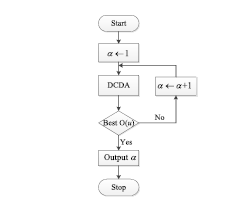
\includegraphics[width=\linewidth]{Figure8.png}
    \caption{Dynamic adjustment of the threshold.}
    \label{fig:8l}
\end{figure}
suspicious URL. Otherwise, it is necessary to further extract
the URL statistical features, the webpage code features and
the webpage text features to combine into multidimensional
features and then perform classification using XGBoost.
It should be noted that if the URL is not accessible, the final
result is also directly given by the CNN-LSTM module. The
description of the DCDA algorithm is as shown follows.
than $\alpha$, then it can be used to directly determine the type of the
\begin{table}[htp]
\begin{tabular}{l}
\hline
\textbf{Algorithm 3} The Dynamic Category Decision Algorithm                                                                                                                                                                                                                         \\ \hline
\textbf{Input:} The suspicious URL $u_{i}$                                                                                           \\
\textbf{Output:} The status of detection                                                                                                                                                              \\
1: $p_{0}$ = LSTM($u_{i}$)                                                                                                                                                                              \\
    
2: $p_{1}$ = 1- $p_{0}$

                            \\
3: $maxi$ = max($p_{0},p_{1}$)                                                                                                                                                                                                                \\
4: $mini$ = min($p_{0},p_{1}$)                                                                                                                                                                                                                                              \\
5: \textbf{if}($maxi|mini > \alpha ||!access(u_{i}))$ \textbf{then}                                                                                                                                                                                                                                                              \\
6: \hspace{4pt} \textbf{if}($p_{1} > p_{0}$) \textbf{then}                                                                                                                                                                                                                                                              \\
7: \hspace{8pt} \textbf{return} $'phishing'$                                                                                                                                                                                                                                              \\
8: \hspace{4pt} \textbf{else return} $'legitimate'$                                                                                                                                                                                        \\
9: \textbf{end if}                                                                                                                                                                                                                                         \\
10: \textbf{end return} multidimensional\_features($u_{i}$)  
                                       \\

11: \textbf{end if}

\\ \hline

\end{tabular}
\end{table}

\section{EVALUATION AND ANALYSIS}
\subsection{EXPERIMENT DATA AND INDICATORS}
The data used in this experiment are real-life data collected
from the Internet. First, historical data confirmed as phishing
from 2014 to 2018 were crawled from the PhishTank website,
and a total of 1 021 758 URLs were used as positive samples
of the phishing. Then, 989 021 URLs were crawled from
the open catalogue website dmoztools.net [38] as negative
samples of the phishing website, which are legitimate URLs.
A total of 2 010 779 URLs were used to set up the dataset
DATA. Because the survival time of the phishing is short,
most of the phishing URLs in DATA are not accessible, it is
impossible to extract the feature of the webpage code and
the text features. To solve this problem, we build the dataset
DATA1 by extracting the currently surviving 22 445 URLs
as phishing from DATA positive samples, and we randomly
select 22 390 accessible URLs from DATA negative samples. The remaining data in DATA are built into the dataset DATA2,
which is $DATA1 \cap DATA2 = \emptyset$ is used to verify
the effectiveness of the multidimensional feature algorithm
and DCDA, and DATA2 is used to verify the effectiveness of
the deep learning algorithm CNN-LSTM. The distribution of
data is shown in Table 3.
\begin{table}[htp]
\caption{Data distribution.}
\label{table:3}
\begin{tabular}{llll}
\hline
dataset & positive & negative & total   \\ \hline
DATA1   & 22445    & 22390    & 44835   \\
DATA2   & 999313   & 966631   & 1965944 \\ \hline
\end{tabular}
\end{table}

\par Let $N_{p}$ indicate the total number of phishing websites, $N_{n}$ indicate the total number of legitimate websites, $N_{p \rightarrow n}$ indicate the phishing websites that were misclassified as
legitimate, $N_{n \rightarrow p}$ indicate the legitimate websites that were
misclassified as phishing, $N_{p \rightarrow p}$ indicate the phishing websites
that were classified as phishing, and $N_{n \rightarrow n}$ indicate the
legitimate websites that were classified as legitimate.We use accuracy, FPR (false positive rate), FNR (false negative rate), cost, and detection time to evaluate the effectiveness of the detection approach we proposed.
\par Accuracy measures the proportion of all correctly classified data out of the total data.
\begin{equation}
\text {Accuracy}=\frac{N_{p \rightarrow p}+N_{n \rightarrow n}}{N_{p}+N_{n}}
\end{equation}
\par FPR (false positive rate) measures the rate of all legitimate
websites that were misclassified as phishing out of the total
legitimate websites.
\begin{equation}
F N R=\frac{N_{p \rightarrow n}}{N_{p}}
\end{equation}
\par FNR (false negative rate) measures the rate of all phishing
websites that were misclassified as phishing out of the total
phishing websites.
\begin{equation}
F N R=\frac{N_{p \rightarrow n}}{N_{p}}
\end{equation}
\par Although misjudging a phishing website as a legitimate website may bring security risks, the number of phishing websites in the real world is far less than the number of legitimate websites, and the risk can be reduced by imparting
phishing knowledge to users. In addition, very small false positive rates may also cause high misidentification. Moreover, a legitimate website misjudged as a phishing website may instill inconvenience and trust issues to the operators of the website. Therefore, we hold the view that the consequences are more serious than the former. We propose the detection cost to comprehensively evaluate FPR and FNR, as follows:
\begin{equation}
\text { cost }=F N R+\lambda \times F P R, \quad \lambda>1
\end{equation}
\par we set $\lambda = 5$
\par The goal of phishing website detection is to find the max
value of O(u), which reduces the false positive rate, the false negative rate and the detection cost and improves the accuracy rate and the detection speed.

\subsection{EXPERIMENT ON THE CNN-LSTM}
This experiment is performed on DATA2 with 5-fold cross-validation. Four sets are used as training sets, the remaining set is used as a test set. First, the parameters of the CNN-LSTM algorithm need to be adjusted. The experiment
finds that the average length of legitimate website samples in dataset DATA is 34.7, the average length of phishing website samples is 87.3, the average length of all the data is 61.5, and the length of URLs exceeding 96.3\% is below 200.
\par Therefore, we set the URL fixed length L = 200. The
average training curve of cross-validation in the CNN-LSTM
is shown in Fig. 9.
\begin{figure}
    \centering
    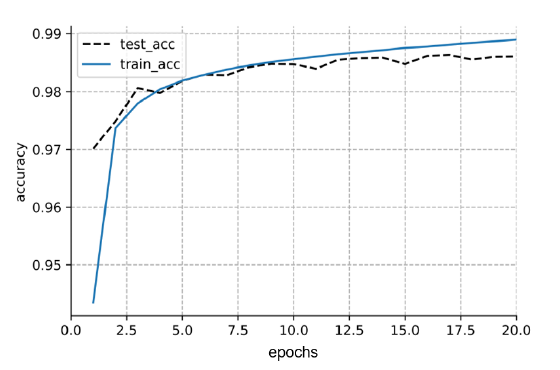
\includegraphics[width=\linewidth]{figure9.png}
    \caption{CNN-LSTM average training curve.}
    \label{fig:9}
\end{figure}

\par When the number of training epochs reaches 20, the accuracy
of the test set is nearly stable; thus, in order to reduce the
training time and prevent overfitting, we set epochs = 20.

\par To verify the effect of the CNN-LSTM algorithm, three
classical deep neural networks, CNN, RNN and LSTM,
are compared in this experiment. The structure of the
CNN-LSTM algorithm is Input->Conv->Maxpool->
LSTM->Softmax. For fairness of the experimental comparison, the network structures of CNN-CNN, RNN-RNN and LSTM-LSTM are compared, whose structure are Input->Conv->Maxpool->Conv->GlobalMaxpool->Softmax, Input->RNN1->RNN2->Softmax, Input->LSTM1-> LSTM2-> Softmax, respectively.
\par We perform calculations on a high-performance server with 64G of memory, a E5-2683 v3 CPU, and GTX 1080ti GPUs, ensuring that deep learning models can be iterated quickly in dealing with large data volumes. The average experimental results for DATA2 are shown in Table 4:
\par From Table 4, Fig. 10 and Fig. 11, the following conclusions can be drawn:
\par The CNN runs at the highest speed, but the detection effect is the worst; the CNN-CNN is slightly slower, and the detection effect is mediocre. The RNN and the RNN-RNN have medium speed, the detection effect is mediocre. The detection

\begin{table}[htp]
\caption{Comparison of different models on DATA2.}
\label{table:4}
\begin{tabular}{llllll}
\hline
Models    & Accuracy/\% & FPR/\% & FNR/\% & Cost/\% & Epoch/s \\ \hline
CNN       & 95.87       & 3.04   & 5.18   & 20.4    & 45      \\
CNN-CNN   & 98.12       & 1.07   & 2.65   & 8.02    & 64      \\
RNN       & 97.87       & 1.46   & 2.78   & 10.09   & 97      \\
RNN-RNN   & 98.71       & 2.12   & 2.47   & 13.05   & 148     \\
LSTM      & 98.42       & 1.18   & 1.97   & 7.87    & 256     \\
LSTM-LSTM & 98.57       & 1.05   & 1.79   & 7.06    & 578     \\
CNN-RNN   & 98.44       & 1.07   & 2.04   & 7.38    & 72      \\
CNN-LSTM  & 98.61       & 0.96   & 1.82   & 6.6     & 140     \\ \hline
\end{tabular}
\end{table}

\begin{figure}
    \centering
    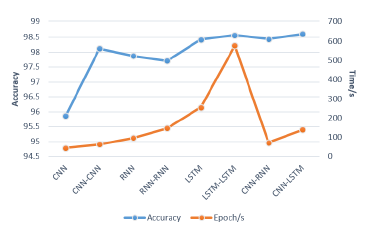
\includegraphics[width=\linewidth]{figure10.png}
    \caption{Accuracy and training time per epoch of different models on
DATA2.}
    \label{fig:10}
\end{figure}

\begin{figure}
    \centering
    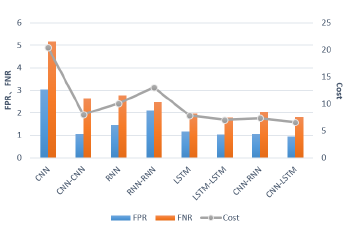
\includegraphics[width=\linewidth]{figure11.png}
    \caption{FPR, FNR and cost of different models on DATA2.}
    \label{fig:11}
\end{figure}

effect of the RNN-RNN is worse than that of RNN, and while
the number of network layers has increased, the evaluation
index does not increase, which indicates that the ``gradient
dispersion'' of the RNN model leads to losses of URL information.
The LSTM and the LSTM-LSTM work better, but each epoch of training requires a large amount of time. The CNN-LSTM model has the highest accuracy and the lowest
detection cost. It has the best detection performance among
all models and the training time is small; therefore, the
CNN-LSTM algorithm is effective.
\par To verify the effect of the CNN-LSTM algorithm in a
big data environment, the CNN-LSTM algorithm is used in 5-fold cross-validation on DATA1 and DATA2. That is, DATA1 and DATA2 are used to train the CNN-LSTM network
respectively, and then, DATA1 is used to test the performance of the network. Since the number of samples in DATA1 is small, the batchsize value is 64.
\par The effect of the two experiments is shown in Fig. 12. It can
be seen that the CNN-LSTM model trained in the DATA2 has better effect on DATA1, which confirms that huge data samples are required for deep learning. However, the effect is worse than the 5-fold cross-validation of the CNN-LSTM algorithm on DATA2, as shown in Table 4, because the samples in DATA1 are currently accessible URLs, whereas the phishing website URLs in DATA2 are historical data and currently inaccessible. Phishing website URLs have different characteristics in different periods due to the different target websites they imitate. Note that the CNN-LSTM model used in the following experiments is trained with DATA2.

\begin{figure}
    \centering
    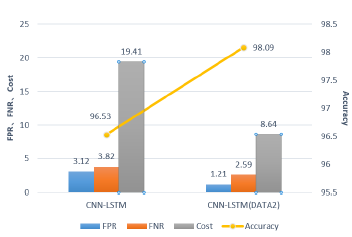
\includegraphics[width=\linewidth]{figure12.png}
    \caption{Experimental comparison of CNN-LSTM on DATA1.}
    \label{fig:12}
\end{figure}

\par Finally, in order to verify the effect of the CNN-LSTM
algorithm compared with traditional phishing URL detection
methods, four methods that AdaBoost, RF (Random Forest),
GBDT and XGBoost are employed to detect phishing URL
based on the 20 statistical URL features. The cross-validation
results ofDATA1 andDATA2 are shown in Fig. 13 and Fig. 14.
It can be seen from the above results that CNN-LSTM is
more effective than traditional phishing URL detection methods.
In addition, XGBoost performs the best among the four
ensemble learning methods.

\begin{figure}
    \centering
    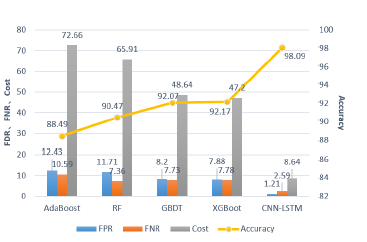
\includegraphics[width=\linewidth]{figure13.png}
    \caption{Comparison with traditional phishing URL detection methods
on DATA1.}
    \label{fig:13}
\end{figure}

\begin{figure}
    \centering
    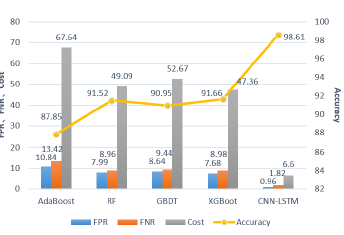
\includegraphics[width=\linewidth]{figure14.png}
    \caption{Comparison with traditional phishing URL detection methods
on DATA2.}
    \label{fig:14}
\end{figure}

\subsection{EXPERIMENT ON THE MULTIDIMENSIONAL FEATURE
ALGORITHM}
The effect of the multidimensional feature algorithm is
verified in this section. After extracting multidimensional
features from DATA1, the experiment results using four
ensemble learning algorithms for classification are shown
in Fig. 15 and Fig. 16. It can be seen that the XGBoost
algorithm has the highest accuracy and the lowest FPR, FNR

\begin{figure}
    \centering
    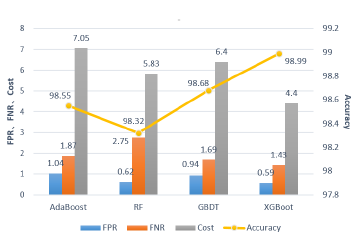
\includegraphics[width=\linewidth]{figure15.png}
    \caption{Four ensemble learning algorithms for classification using
multidimensional features..}
    \label{fig:15}
\end{figure}

\begin{figure}
    \centering
    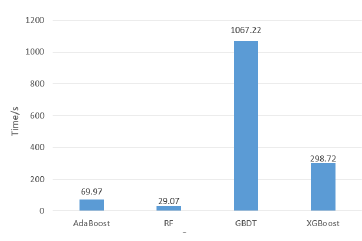
\includegraphics[width=\linewidth]{figure16.png}
    \caption{Training time of four ensemble learning algorithms using
multidimensional features.}
    \label{fig:16}
\end{figure}
and cost compared with AdaBoost, random forest and GBDT;
it also has a faster training speed than GBDT.
\par In addition, XGBoost is applied to the phishing website
detection method based on the traditional feature, which is
the statistical feature according to the Table 2, compared with
CNN-LSTM and the multidimensional features, as shown
in Fig. 17. It can be seen that the multidimensional feature
algorithm signicantly improves the accuracy and reduces
FPR, FNR and cost compared with CNN-LSTM and the
traditional feature extraction method.
\begin{figure}
    \centering
    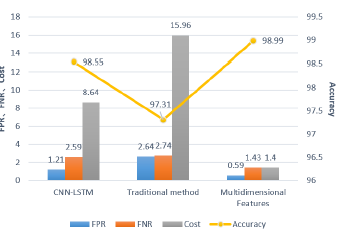
\includegraphics[width=\linewidth]{figure17.png}
    \caption{Comparison of the traditional feature method, CNN-LSTM and
the multidimensional feature algorithm.}
    \label{fig:17}
\end{figure}
Table 5 illustrates the three metrics of MFPD and
other approaches (Mao et al. [11], CANTINA+ [19],
Bahnse et al. [32]) based on the evaluation value in the papers.
In order to facilitate comparison, we calculate the three metrics
based on our experiment results. Bahnse et al. [32] has
highest recall than MFPD, but MFPD achieves the highest
precision and F1. Because the detection process of our
approach relies on the hybrid features, which are obtained
from multiple aspects and have more information than the
features from a single aspect, and it utilizes millions of data
for training.

\subsection{EXPERIMENT ON THE DYNAMIC CATEGORY
DECISION ALGORITHM}
In this section, we conduct five-fold cross validation on
DATA1 to prove the validity of the dynamic category decision
algorithm DCDA. The key of DCDA is to find the optimal
threshold $\alpha$ so that it can quickly detect phishing websites
with high accuracy and low detection cost.
The experiment results are shown in Fig. 18 and Fig. 19.
When a threshold of approximately $\alpha = 355$, the detection
\begin{figure}
    \centering
    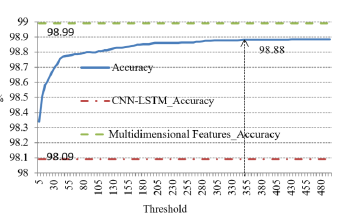
\includegraphics[width=\linewidth]{figure18.png}
    \caption{DCDA algorithm accuracy rate curve.}
    \label{fig:18}
\end{figure}

\begin{figure}
    \centering
    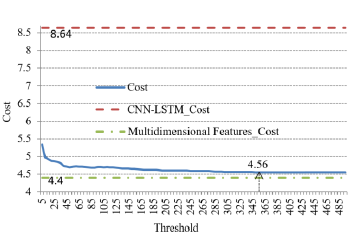
\includegraphics[width=\linewidth]{figure19.png}
    \caption{DCDA algorithm detection cost curve.}
    \label{fig:19}
\end{figure}
accuracy and the detection cost tend to be stable, reaching
98.88\% and 4.56, which is almost equivalent to the multidimensional
feature detection. The most important role of DCDA is real-time detection. Fig. 20 shows that as the threshold increases, the average number of websites that
CNN-LSTM is responsible for detecting gradually decreases, and the number of websites that the multidimensional feature detection is responsible for detecting gradually increases. When the threshold is approximately The preferred spelling of
$\alpha = 355$ only 28\% of the websites need to undergo the multidimensional feature detection, which greatly reduces the workload.
\begin{figure}
    \centering
    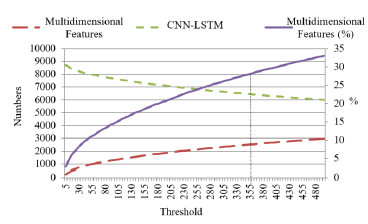
\includegraphics[width=\linewidth]{figure20.png}
    \caption{Detection number curve under different thresholds.}
    \label{fig:20}
\end{figure}

\par It is found in the experiment that the time taken by the CNN-LSTM algorithm to predict the entire test set does not exceed 10 s. The multidimensional feature algorithm has an average detection time of 3.5 s for per URL due to the need to extract the code features of the webpage, the text features of the web page, and the WHOIS information in the URL features. For convenience, we set the average length of CNN-LSTM website detection to 0.5 s and the number of data samples from DATA1 to 10 000. The experimental result is shown in Fig. 21. As the threshold increases, the average detection time of the DCDA algorithm changes linearly.
When the threshold $\alpha = 355$, the average detection time is less than one-half of the multidimensional feature detection.
\begin{figure}
    \centering
    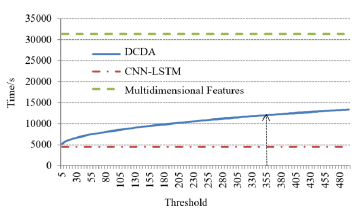
\includegraphics[width=\linewidth]{figure21.png}
    \caption{DCDA detection time curve.}
    \label{fig:21}
\end{figure}
\par In summary, considering detection accuracy, detection cost
and detection time, the threshold of the DCDA algorithm
is set to 355, which guarantees appropriate accuracy and
detection cost of phishing website detection and significantly
reduces the detection time.

\section{CONCLUSION}
It is well known that a good phishing website detection
approach should have good real-time performance while
ensuring good accuracy and a low false positive rate. Our proposed
MFPD approach is consistent with this idea. Under the
control of a dynamic category decision algorithm, the URL
character sequence without phishing prior knowledge ensures
the detection speed, and the multidimensional feature detection
ensures the detection accuracy. We conduct a series of
experiments on a dataset containing millions of phishing and
legitimate URLs. From the results, we find that the MFPD
approach is effective with high accuracy, low false positive
rate and high detection speed. A future development of our
approach will consider applying deep learning to feature
extraction of webpage code and webpage text. In addition, we
plan to implement our approach into a plugin for embedding
in a Web browser.

\begin{thebibliography}{00}

\bibitem{b1} Phishing Attack Trends Re-Port-1Q. Accessed: May 5, 2018.
[Online]. Available: https://apwg.org/resources/apwg-reports/

\bibitem{b2} Kaspersky Security Bulletin: Overall Statisticals For. Accessed:
Jul. 12, 2018. [Online]. Available: https://securelist.com/ksb-overallstatistics-
2017/83453/

\bibitem{b3} A.Y. Ahmad, M. Selvakumar, A. Mohammed, and A.-S. Samer, ``TrustQR:
A new technique for the detection of phishing attacks on QR code,'' Adv.
Sci. Lett., vol. 22, no. 10, pp. 2905-2909, Oct. 2016.

\bibitem{b4} C. C. Inez and F. Baruch, ``Setting priorities in behavioral interventions: An application to reducing phishing risk,'' Risk Anal., vol. 38, no. 4, pp. 826-838, Apr. 2018.

\bibitem{b5} G. Diksha and J. A. Kumar, ``Mobile phishing attacks and defence mechanisms: State of art and open research challenges,'' Comput. Secur., vol. 73,
pp. 519-544, Mar. 2018.

\bibitem{b6} \textit{Google Safe Browsing APIs}. Accessed: Oct. 1, 2018. [Online]. Available: https://developers.google.com/safe-browsing/v4/

\bibitem{b7} S. Sheng, B. Wardman, G. Warner, L. Cranor, J. Hong, and C. Zhang,
``An empirical analysis of phishing blacklists,'' in Proc. 6th Conf. Email
Anti-Spam (CEAS), Jul. 2009, pp. 59-78.

\bibitem{b8} A. K. Jain and B. B. Gupta, ``A novel approach to protect against phishing attacks at client side using auto-updated white-list,'' EURASIP J. Inf.
Secur., vol. 2016, no. 1, Dec. 2016, Art. no. 34.

\bibitem{b9} M. Zouina and B. Outtaj, ``A novel lightweight URL phishing detection
system using SVM and similarity index,'' Hum.-Centric Comput. Inf. Sci.,
vol. 7, no. 1, p. 17, Jun. 2017.

\bibitem{b10} E. Buber, Ö. Demir, and O. K. Sahingoz, ``Feature selections for the
machine learning based detection of phishing websites,'' in Proc. IEEE
Int. Artif. Intell. Data Process. Symp. (IDAP), Sep. 2017, pp. 1-5.

\bibitem{b11} J. Mao et al., ``Detecting phishing websites via aggregation analysis of page layouts,'' Procedia Comput. Sci., vol. 129, pp. 224-230, Jan. 2018.

\bibitem{b12} J. Mao,W. Tian, P. Li, T.Wei, and Z. Liang, ``Phishing-alarm: Robust and efficient phishing detection via page component similarity,'' IEEE Access,
vol. 5, no. 99, pp. 17020-17030, Aug. 2017.

\bibitem{b13} J. Cao, D. Dong, B. Mao, and T. Wang, ``Phishing detection method
based on URL features,'' J. Southeast Univ.-Engl. Ed., vol. 29, no. 2,
pp. 134-138, Jun. 2013.

\bibitem{b14} S. C. Jeeva and E. B. Rajsingh, ``Phishing URL detection-based feature selection to classifiers,'' Int. J. Electron. Secur. Digit. Forensics, vol. 9, no. 2, pp. 116-131, Jan. 2017.

\bibitem{b15} A. Le, A. Markopoulou, and M. Faloutsos, ``PhishDef: URL names say it all,'' in Proc. IEEE Int. Conf. Comput. Commun. (INFOCOM), Sep. 2010,
pp. 191-195.

\bibitem{b16} R. Verma and K. Dyer, ``On the character of phishing URLs: Accurate and
robust statisticalal learning classifiers,'' in Proc. 5th ACMConf. Data Appl.
Secur. Priv. (ACM CODASPY), Mar. 2015, pp. 111-122.

\bibitem{b17} Y. Li, S. Chu, and R. Xiao, ``A pharming attack hybrid detection
model based on IP addresses and Web content,'' Optik, vol. 126, no. 2,
pp. 234-239, Nov. 2014.

\bibitem{b18} G. G. Xiang and J. Hong, ``A hybrid phish detection approach by identity discovery and keywords retrieval,'' in Proc. Int. Conf. World Wide Web
(WWW), Oct. 2009, pp. 571-580

\bibitem{b19} G. Xiang, J. Hong, C. P. Rose, and L. Cranor, ``CANTINAC: A featurerich
machine learning framework for detecting phishing Web sites,'' ACM
Trans. Inf. Syst. Secur., vol. 14, no. 2, p. 21, Sep. 2011.

\bibitem{b20} S. Marchal, K. Saari, N. Singh, and N. Asokan, ``Know your phish: Novel
techniques for detecting phishing sites and their targets,'' in Proc. IEEE
36th Int. Conf. Distrib. Comput. Syst. (ICDCS), Jun. 2016, pp. 323-333.

\bibitem{b21} R. Patil, B. D. Dhamdhere, K. S. Dhonde, and R. G. Chinchwade,
``A hybrid model to detect phishing-sites using clustering and Bayesian
approach,'' in Proc. IEEE Int. Conf. Converg. Technol. (I2CT), Apr. 2014,
pp. 1-5.

\bibitem{b22} M. Arab and M. K. Sohrabi, ``Proposing a new clustering method to detect
phishing websites,'' Turkish J. Electr. Eng. Comput. Sci., vol. 15, no. 1,
pp. 92-95, Jun. 2015.

\bibitem{b23} A. Shinde, A. Pandey, R. Pawar, and V. Gangule, ``Clustering and Bayesian
approach-based model for detection of phishing,'' Int. J. Comput. Appl.,
vol. 118, no. 24, pp. 30-33, May 2015.

\bibitem{b24} X. Zhang, Z. Yan, H. Li, and G. Geng, ``Research of phishing detection
technology,'' Chin. J. Netw. Inf. Secur., vol. 3, no. 7, pp. 7-24, Jul. 2017.

\bibitem{b25} J. Ma, L. K. Saul, S. Savage, and G. M. Voelker, ``Beyond blacklists:
Learning to detect malicious web sites from suspicious URLs,'' in Proc.
15th ACM SIGKDD Int. Conf. Knowl. Discover Data Mining (KDD),
Jan. 2009, pp. 1245-1254.

\bibitem{b26} R. M. Mohammad, F. Thabtah, and L. Mccluskey, ``Predicting phishing
websites based on self-structuring neural network,'' Neural Comput. Appl.,
vol. 25, no. 2, pp. 443-458, Aug. 2014.

\bibitem{b27} A. K. Jain and B. B. Gupta, ``Towards detection of phishing websites on
client-side using machine learning based approach,'' Telecommun. Syst.,
vol. 68, no. 4, pp. 687-700, Aug. 2018.

\bibitem{b28} J. Zhang, Y. Ou, D. Li, and Y. Xin, ``A prior-based transfer learning
method for the phishing detection,'' J. Netw., vol. 7, no. 8, pp. 1201-1207,
Aug. 2012.

\bibitem{b29} L. Chang et al., ``Convolutional neural networks in image understanding,''
Acta. Automatica Sinica, vol. 42, no. 9, pp. 1300-1312, Jul. 2016.

\bibitem{b30} Z. C. Lipton, J. Berkowitz, and C. Elkan. (Oct. 2015). ``A critical review
of recurrent neural networks for sequence learning.'' [Online]. Available:
https://arxiv.org/abs/1506.00019

\bibitem{b31} S. G. Selvaganapathy, M. Nivaashini, and H. P. Natarajan, ``Deep belief
network based detection and categorization of malicious URLs,'' Inf. Secur.
J., Global Perspective, vol. 27, no. 3, pp. 145-161, Apr. 2018.

\bibitem{b32} A. C. Bahnse, E. C. Bohorquez, S. Villegas, J. Vargas, and F. A. Gonález,
``Classifying phishing URLs using recurrent neural networks,'' in Proc.
IEEE APWG Symp. Electron. Res. (eCrime), Apr. 2017, pp. 1-8.

\bibitem{b33} X. Zhang, J. Zhao, and Y. LeCun, ``Character-level convolutional networks
for text classification,'' in Proc. 28th Int. Conf. Neural Inf. Process. Syst.
(NIPS), Dec. 2015, pp. 649-657.

\bibitem{b34} Y. Xiao and K. Cho. (Feb. 2016). ``Efficient character-level document
classification by combining convolution and recurrent layers.'' [Online].
Available: https://arxiv.org/abs/1602.00367

\bibitem{b35} G. Hinton, N. Srivastava, A. Krizhevsky, I. Sutskever, and
R. Salakhutdinov. (Jul. 2012). ``Improving neural networks by
preventing co-adaptation of feature detectors.'' [Online]. Available:
https://arxiv.org/abs/1207.0580

\bibitem{b36} N. Srivastava, G. Hinton, A. Krizhevsky, I. Sutskever, and
R. Salakhutdinov, ``Dropout: A simple way to prevent neural networks
from overdfitting,'' J. Mach. Learn. Res., vol. 15, no. 1, pp. 1929-1958,
Jun. 2014.

\bibitem{b37} D. P. Kingma and J. Ba. (Dec. 2014). ``Adam: A method for stochastic
optimization.'' [Online]. Available: https://arxiv.org/abs/1412.6980

\bibitem{b38} A Open-Content Directory of World Wide Web Links. Accessed:
Oct. 12, 2018. [Online]. Available: https://dmoztools.net/
\end{thebibliography}

\begin{IEEEbiography}[{
\includegraphics[width=1in,height=1.25in,clip,keepaspectratio]{author1.png}}]{Penny Yang} (M'76--SM'81--F'87) received the Ph.D. degree from Southeast University, in 2006. He was with CERN as a Research 
Scientist to take part in the Alpha Magnetic Spectrometer Experiment from 2007 to 2009, which was led by Nobel Laureate Prof. S. Ting. 
He is currently an Associate Professor with the School of Computer Science and Engineering, Southeast University. His research interests include new generation Internet architecture, network security, and cyber content governance. He is the Deputy Director of the Future Network Research Center, Southeast University, and a member of the National Technical Committee of
Standardization Administration of China.
\end{IEEEbiography}

\begin{IEEEbiography}[{
\includegraphics[width=1in,height=1.25in,clip,keepaspectratio]{author2.png}}]{GUANGZHEN ZHAO} received the B.S. and M.S. degrees from the School of Information Science and Technology, Shijiazhuang Tiedao University, China, in 2015 and 2018, respectively. He is currently pursuing the Ph.D. degree with the School of Computer Science and Engineering, Southeast University. His current research interests include network security, situation awareness, and new
generation Internet architecture.
\end{IEEEbiography}

\begin{IEEEbiography}[{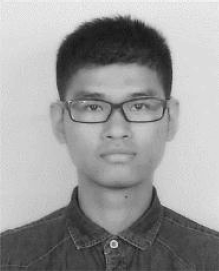
\includegraphics[width=1in,height=1.25in,clip,keepaspectratio]{author3.png}}]{PENG ZENG} (M'87) received the B.S. degree from the
Wuhan University of Science and Technology,
Wuhan, China, in 2015, and the M.S. degree from
Southeast University, Nanjing, China, in 2018.
His research interests include Web security,
cloud computing, and new generation Internet
architecture.
\end{IEEEbiography}

\EOD

\end{document}
